% 第一节

\section{滕王阁序}
\subsection{二级标题}
\subsubsection{第一段}

豫章故郡,洪都新府。星分翼轸,地接衡庐。襟三江而带五湖,控蛮荆而引瓯越。物华天宝,龙光射牛斗之墟;人杰地灵,徐孺下陈蕃之榻。雄州雾列,俊采星驰。台隍枕夷夏之交,宾主尽东南之美。都督阎公之雅望,棨戟遥临;宇文新州之懿范,襜帷暂驻。十旬休假,胜友如云;千里逢迎,高朋满座。腾蛟起凤,孟学士之词宗;紫电青霜,王将军之武库。家君作宰,路出名区;童子何知,躬逢胜饯。

\begin{figure}[htb]
    \centering
    \subfigure[$y=\sinh(x)$]{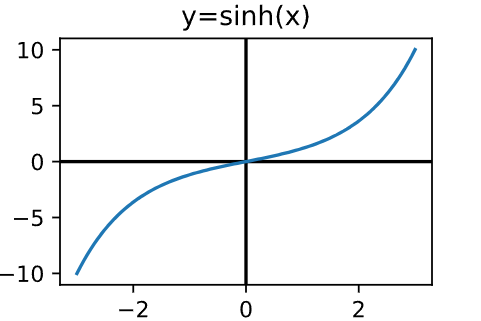
\includegraphics[width=0.3\linewidth]{./res/sinh.drawio.png}}\;
    \subfigure[$y=\sin(x)$]{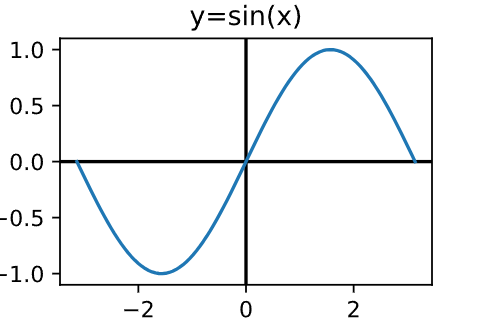
\includegraphics[width=0.3\linewidth]{./res/sin.drawio.png}}\\
    \subfigure[$y=\tan(x)$]{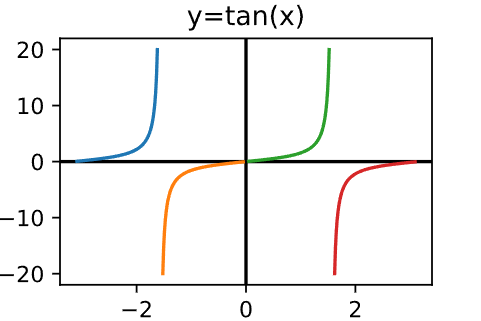
\includegraphics[width=0.3\linewidth]{./res/tan.drawio.png}}\;
    \subfigure[$y=\log(x)$]{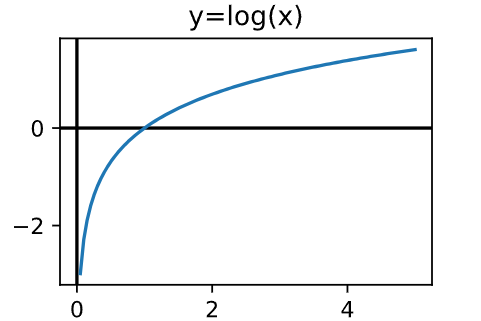
\includegraphics[width=0.3\linewidth]{./res/log.drawio.png}}

    \caption{函数图像}
    \label{fig:test}
\end{figure}

时维九月,序属三秋。潦水尽而寒潭清,烟光凝而暮山紫。俨骖騑于上路,访风景于崇阿;临帝子之长洲,得天人之旧馆。层峦耸翠,上出重霄;飞阁流丹,下临无地。鹤汀凫渚,穷岛屿之萦回;桂殿兰宫,即冈峦之体势。

\begin{table}[htb]
    \centering
    \caption{超声波实验数据}
    \label{tab:test}
    \begin{tabular}{|c|*{6}{c|}}
        \hline
        &\multicolumn{2}{c|}{第一组}&\multicolumn{2}{c|}{第二组}&\multicolumn{2}{c|}{第三组}\\
        \hline
        \makecell{采样频率}&\makecell{时间 1}&\makecell{时间 2}&\makecell{时间 3}&\makecell{时间 4}&\makecell{时间 5}&\makecell{时间 6}\\
        \hline
        \makecell{10000 Hz}&\makecell{0.0118 s}&\makecell{0.0131 s}&\makecell{0.0242 s}&\makecell{0.0257 s}&\makecell{0.0367 s}&\makecell[c]{0.0380 s}\\
        \hline
    \end{tabular}
\end{table}

\subsubsection{第二段}
披绣闼,俯雕甍,山原旷其盈视,川泽纡其骇瞩。闾阎扑地,钟鸣鼎食之家;舸舰弥津,青雀黄龙之舳。云销雨霁,彩彻区明。落霞与孤鹜齐飞,秋水共长天一色。渔舟唱晚,响穷彭蠡之滨;雁阵惊寒,声断衡阳之浦。

\begin{itemize}
    \item item1
    \item item2
    \begin{itemize}
        \item subitem1
        \item subitem2
    \end{itemize}
    \item item3
    \begin{enumerate}
        \item subitem3
        \item subitem4
    \end{enumerate}
\end{itemize}

遥襟甫畅,逸兴遄飞。爽籁发而清风生,纤歌凝而白云遏。睢园绿竹,气凌彭泽之樽;邺水朱华,光照临川之笔。四美具,二难并。穷睇眄于中天,极娱游于暇日。天高地迥,觉宇宙之无穷;兴尽悲来,识盈虚之有数。

\subsection{第二部分}
\subsubsection{第三段}
望长安于日下,目吴会于云间。地势极而南溟深,天柱高而北辰远。关山难越,谁悲失路之人?萍水相逢,尽是他乡之客。怀帝阍而不见,奉宣室以何年?

嗟乎!时运不齐,命途多舛。冯唐易老,李广难封。屈贾谊于长沙,非无圣主;窜梁鸿于海曲,岂乏明时?所赖君子见机,达人知命。老当益壮,宁移白首之心?穷且益坚,不坠青云之志。酌贪泉而觉爽,处涸辙以犹欢。北海虽赊,扶摇可接;东隅已逝,桑榆非晚。孟尝高洁,空余报国之情;阮籍猖狂,岂效穷途之哭!

\begin{equation}
    \label{equ:test}
    A=U\Sigma V^T=\begin{bmatrix}\frac{1}{\sqrt{5}}&\frac{-2}{\sqrt{5}}\\\frac{2}{\sqrt{5}}&\frac{1}{\sqrt{5}}\end{bmatrix}\begin{bmatrix}\sqrt{125}&0\\0&0\end{bmatrix}\begin{bmatrix}0.8&0.6\\0.6&-0.8\end{bmatrix}
\end{equation}

\subsubsection{第四段}
勃,三尺微命,一介书生\cite{book:test}。无路请缨,等终军之弱冠\cite{mt:test};有怀投笔,慕宗悫之长风。舍簪笏于百龄,奉晨昏于万里。非谢家之宝树,接孟氏之芳邻。他日趋庭,叨陪鲤对;今兹捧袂,喜托龙门。杨意不逢,抚凌云而自惜;钟期既遇,奏流水以何惭?

呜乎!胜地不常\cite{article:test},盛筵难再;兰亭已矣,梓泽丘墟。临别赠言\cite{ol:test},幸承恩于伟饯;登高作赋,是所望于群公。敢竭鄙怀,恭疏短引;一言均赋,四韵俱成。请洒潘江,各倾陆海云尔:
